\section{Constructing the MQL algebra tree}
The MQL queries are constructed as a tree of operators bottom-up while parsing
the abstract syntax tree (for the corresponding XQuery query). 

\subsection{Operators and parameters}
\begin{figure}[!htp]
\begin{center}
  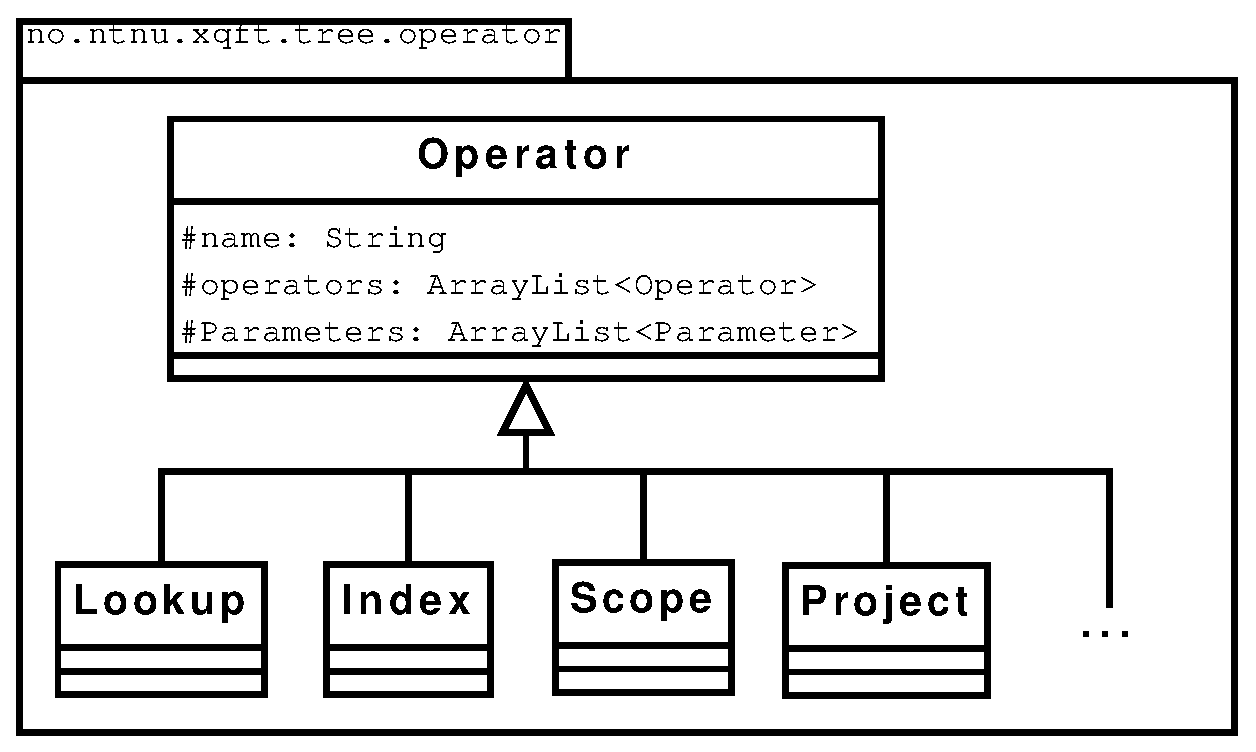
\includegraphics[scale=0.4]{diagrams/mql_operator_uml}
  \caption{Simplified class diagram of MQL operators}
  \label{fig:impl:mql_op_uml}
\end{center}
\end{figure}
The operators modeled in the implementation correspond to the operators
described in section \ref{sect:method:marsOperators}. A simplified class
diagram is shown in figure \ref{fig:impl:mql_op_uml}. Note that the
responsibility with regards to converting an operator to a string
representation is largely left to the various subclasses. However, the default
fallback for the \texttt{Operator} class is to return a string of the form
\begin{Verbatim}
operator_name(param1, param2, ..., paramN; 
              operator1, operator2, ..., operatorM)
\end{Verbatim}
This is sufficient in some cases, such as for the model of the \texttt{cross()}
operator.

\begin{figure}[!htp]
\begin{center}
  \includegraphics[scale=0.4]{diagrams/mql_param_uml}
  \caption{Class diagram of MQL parameters}
  \label{fig:impl:mql_param_uml}
\end{center}
\end{figure}

MQL arameters (as described in \ref{sect:method:mql:concepts}) are modelled as
seen in figure \ref{fig:impl:mql_param_uml}. Parameters require no complex
structure, and are only created and added to operators as needed.

\subsection{Concepts}
As mentioned, MQL queries are represented as trees, where each node represents
an operator. Each node is an instance of an operator class (as described
above), and contains a list of child operators and a list of parameters. To
convert the operator tree to a MQL query string, simply call the method
\texttt{toPrettyString(0)} on the root node of the operator tree.

\subsection{Usage}
The operator classes are designed to be intuitive and simple to use. Figure
\ref{fig:impl:mql_op_ex1_java} shows one example where a simple operator tree
is built and converted to an MQL query string (the result of which can be seen
in figure \ref{fig:impl:mql_op_ex1_mql}).

%\usepackage{graphics} is needed for \includegraphics
\begin{figure}[htp]
\begin{center}
  \begin{Verbatim}
Lookup lookup = new Lookup("Death in the clouds");
Scope scope = new Scope("/books/book/title", lookup);
Project project = new Project("author", scope);
System.out.println(project.toPrettyString(0));
  \end{Verbatim}
  \caption{Example java code to construct a MQL operator tree}
  \label{fig:impl:mql_op_ex1_java}
\end{center}
\end{figure}

\begin{figure}[htp]
\begin{center}
  \begin{Verbatim}
project([author];
  scope(/books/book/title;
    lookup("Death in the clouds")))
  \end{Verbatim}
  \caption{Resulting MQL query string from example in figure
  \ref{fig:impl:mql_op_ex1_java}}
  \label{fig:impl:mql_op_ex1_mql}
\end{center}
\end{figure}
